\subsection{The Purpose of Neural Networks for Image Processing}

Neural networks in image processing aim to emulate the visual system of animals (\cref{fig:nn-purpose-zebra}), creating algorithmic analogies to the physical neuronal pathways used in visual perception.
In the human brain, many aspects of our visual system, such as the ability to interpret images regardless of their orientation and extrapolate from known information, are often taken for granted.
However, replicating these capabilities algorithmically poses significant challenges.
Neural networks alleviate the need for manual feature selection, which has been a limitation of traditional image processing methods.
This automation not only simplifies the process but also enhances the ability of these systems to interpret and process images in ways similar to the human brain, making neural networks a powerful tool in the realm of image processing.


\begin{figure}[h!]
  \centering
  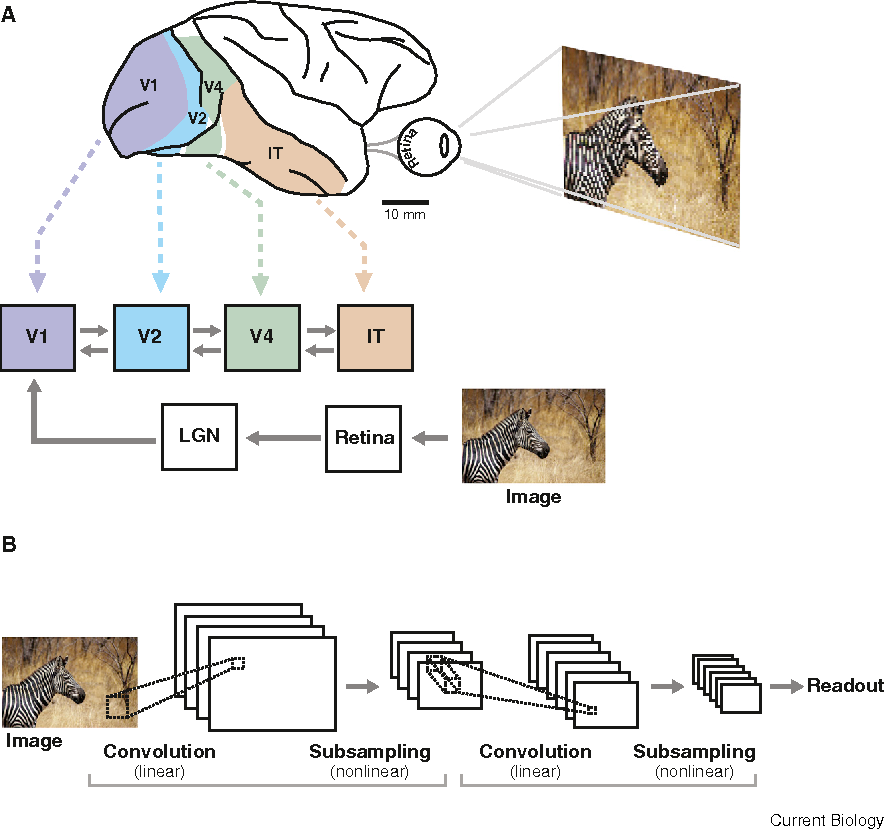
\includegraphics[width = 0.75\linewidth]{figures/raster/visual-nn.png}
  \caption{An example of a neural network mimicking the human brain.}
  \label{fig:nn-purpose-zebra}
\end{figure}

%%% Local Variables:
%%% mode: latex
%%% TeX-master: "../../../Andrew_Jensen_Dissertation"
%%% End:
